\section{From double categories to bicategories}
\label{sec:1x1-to-bicat}

We are now equipped to lift structures on double categories to
their loose bicategories.  In this section we show that passage
from double categories to bicategories is given by a functor of locally cubical bicategories. In order to prove this, we first give an intermediate result that $\cH$ lifts to a functor of hom-bicategories
\begin{align}
    \cDbl(\lD,\lE) &\too \cBicat(\cH(\lD),\cH(\lE))\\
\end{align}

As a point of notation, we write $\odot$ for the composition of
1-cells in a bicategory, since our bicategories are generally of the
form $\cH(\lD)$.  As advocated by Max Kelly, we say \textbf{functor}
to mean a morphism between bicategories that preserves composition up
to isomorphism; equivalent terms include \emph{weak 2-functor},
\emph{pseudofunctor}, and \emph{homomorphism}.

Recall that the assignment $\cH$ sends each double category $\lC$ to the loose bicategory  $\cH(\lD)$ of objects, 1-cells, and globular 2-morphisms of $\lD$.  Note that functors of double categories and bicategories compose strictly associatively; hence, we can talk about the 1-categories of double categories and bicategories, which we denote ${\bf Dbl}$ and ${\bf Bicat}$ respectively.

\begin{thm}\label{thm:1-func}
 If \lD\ is a double category, then $\cH(\lD)$ is a bicategory, and
  any functor $F\maps \lD\to\lE$ induces a functor $\cH(F)\maps
  \cH(\lD)\to\cH(\lE)$.  In this way $\cH$ defines a functor of
  1-categories $\mathbf{Dbl}\to \mathbf{Bicat}$.
\end{thm}
\begin{proof}
 The constraints of $F$ are all globular, hence give constraints for
  $\cH(F)$.  Functoriality is evident.
\end{proof}

% MS: This doesn't really make precise sense, and I'm not sure it's necessary.
%Note that this is a stronger condition than we need for our main result.
The action of \cH\ on transformations is less obvious. It
requires the presence of companions or conjoints, to lift the part of the data given by vertical morphisms to loose 1-cells. Before we discuss how this works, we briefly recall some definitions regarding transformations between functors of bicategories.

If $F,G\maps \cA\to\cB$ are functors between bicategories, then an
\textbf{oplax transformation} $\al\maps F\to G$ consists of 1-cells
$\al_A\maps FA\to GA$ and 2-cells
\[\vcenter{\xymatrix{ \ar[r]^{Ff}\ar[d]_{\al_A} \drtwocell\omit{\al_f} &  \ar[d]^{\al_B}\\
  \ar[r]_{Gf} & }}\]
such that for any 2-cell $\xymatrix{A \rtwocell^f_g{x} & B}$ in \cA,
\begin{equation}
  \label{eq:laxtransf-nat}
  \vcenter{\xymatrix@R=1pc@C=3pc{
      \rtwocell^{Ff}_{Fg}{Fx}\ar[dd]_{\al_A} 
      &  \ar[dd]^{\al_B}\\
      \drtwocell\omit{\al_g} & \\
      \ar[r]_{Gg} & }}\;=\;
  \vcenter{\xymatrix@R=1pc@C=3pc{
      \ar[r]^{Ff}\ar[dd]_{\al_A} \drtwocell\omit{\al_f} &
      \ar[dd]^{\al_B}\\ & \\
      \rtwocell^{Gf}_{Gg}{Gx} & }}
\end{equation}
and moreover for any $A$ and any $f,g$ in \cA,
\begin{equation}
  \vcenter{\xymatrix@R=5pc{
      \rtwocell^{1_{FA}}_{F(1_A)}{\iso} \ar[d]_{\al_A} \drtwocell\omit{\al_{1_A}} &  \ar[d]^{\al_A}\\
      \rtwocell^{G(1_A)}_{1_{GA}}{\iso} & }} \;=\;
  \vcenter{\xymatrix{ \ar[r]^{1_{FA}}\ar[d]_{\al_A} \drtwocell\omit{\iso}&  \ar[d]^{\al_A}\\
      \ar[r]_{1_{GA}} &
    }}
  \quad\text{and}\quad
  \vcenter{\xymatrix{
      \ar[r]|{Ff}\ar[d]_{\al_A} \drtwocell\omit{\al_f}
      \rruppertwocell^{F(gf)}{\iso}
      &
      \ar[r]|{Fg}\ar[d]|{\al_B} \drtwocell\omit{\al_g} &
      \ar[d]^{\al_C}\\
      \ar[r]|{Gf} \rrlowertwocell_{G(gf)}{\iso} & \ar[r]|{Gg} & }}
  \;=\;
  \vcenter{\xymatrix{ \ar[r]^{F(gf)}\ar[d]_{\al_A} \drtwocell\omit{\al_{gf}} &  \ar[d]^{\al_C}\\
      \ar[r]_{G(gf)} & }}\label{eq:laxtransf-ax}
\end{equation}
It is a \textbf{lax transformation} if the 2-cells $\al_f$ go the
other direction, and a \textbf{pseudo transformation} if they are
isomorphisms.

Inverses of morphisms in a category are unique when they exist, so for a morphism (and in particular a natural transformation) to be an isomorphism is only a property rather than a structure.
But since inverse equivalences of morphisms in a bicategory are unique only up to isomorphism, if we only know that a morphism has the property of being an equivalence, we have to make choices to find an inverse equivalence.
For many purposes (see e.g.~\cite{nick:tricats}) it is more useful to include a ``coherent'' inverse equivalence as specified data so that such choices are no longer necessary; in the case of transformations the result is called a pseudo natural adjoint equivalence.

Before defining these, we first consider a more general notion of ``conjunctonal transformation.''
By doctrinal adjunction~\cite{kelly:doc-adjn}, given collections of
1-cells $\al_A\maps FA\to GA$ and $\be_A\maps GA\to FA$ and
adjunctions $\al_A\adj \be_A$ in \cB, there is a bijection between
\begin{inparaenum}
\item collections of 2-cells $\al_f$ making $\al$ an oplax
  transformation and
\item collections of 2-cells $\be_f$ making $\be$ a lax
  transformation.
\end{inparaenum}
Two such transformations correspond under this bijection if and only if
\begin{equation}
  \vcenter{\xymatrix@-.5pc{F(f) \ar[r]^-{\eta \odot \mbox{\tiny id}_{F(f)}}
      \ar[d]_{\mbox{\tiny id}_{F(f)}\odot \eta} &
      \be_B\odot \al_B \odot F(f) \ar[d]^{\mbox{\tiny id}_{\be_B} \odot \al_f}\\
      F(f) \odot \be_A\odot \al_A\ar[r]_-{\be_f \odot \mbox{\tiny id}_{\al_A}} &
      \be_B\odot G(f) \odot \al_A}}
  \quad\text{and}\quad
  \vcenter{\xymatrix@-.5pc{\al_B\odot F(f)\odot \be_A
      \ar[r]^-{\mbox{\tiny id}_{\al_B}\odot \be_f}\ar[d]_{\al_f \odot \mbox{\tiny id}_{\be_A}}&
      \al_B \odot \be_B \odot G(f)\ar[d]^{\ep \odot \mbox{\tiny id}_{G(f)}}\\
      G(f)\odot \al_A\odot \be_A \ar[r]_-{\mbox{\tiny id}_{G(f)} \odot \ep} & G(f)}}\label{eq:conjtrans}
\end{equation}

%In planar diagrams, this looks like
%\begin{align}
%\begin{tikzpicture}[scale=1.75]
%\draw[fill=blue, draw=blue] (-1,0) -- (-1,-1.4) -- (-.6,-1.4) -- (-.6,0) -- (-1,0);
%\draw[fill=red, draw=red] (-.6,0) -- (-.6,-1.4) -- (0,-1.4) -- (0,0) -- (-.6,0);  
%\draw[fill=blue, draw=blue] (-1,-1.4) -- (-1,-2) -- (.6,-2) -- (.6,-1.4) -- (-1,-1.4);  
%\draw[fill=green, draw=green] (.6,-.6) -- (0,-.6) -- (0,0) -- (.6,0) -- (.6,-.6); 
%\draw[fill=blue, draw=blue] (.6,-.6) -- (1,-.6) -- (1,0) -- (.6,0) -- (.6,-.6); 
%\draw[fill=blue, draw=blue] (0,-.6) -- (.6,-.6) -- (.6,-2) -- (0,-2) -- (0,-.6); 
%\draw[fill=yellow, draw=yellow] (.6,-2) -- (1,-2) -- (1,0) -- (.6,0) -- (.6,-2); 
 %    \draw (.6,-.6) to (.6,0);
  %   \draw (0,-1.4) to (0,0);
   %   \draw (-.6,-1.4) to (-.6,0);
  %     \node[morphism, minimum width=20mm] (l) at (-.3,-1.4) {$\eta$};
   %    \node[morphism, minimum width=20mm] (r) at (.3,-.6) {$\beta_f$};
%\draw (-.3, -2) to (l.south);
  %  \end{tikzpicture}
%\end{align}

commute.  If we have a pointwise adjunction between an oplax and a lax
transformation, whose 2-cell structures correspond under this
bijection, we call it a \textbf{conjunctional transformation}
$(\al\conj \be)\maps F\to G$.  (These are the conjoint pairs in a
double category whose loose arrows are lax transformations and
whose vertical arrows are oplax transformations.)

Of particular importance is the case when both $\al$ and \be\ are
pseudo natural and each adjunction $\al_A\adj \be_A$ is an adjoint
equivalence.  In this case we call $\al\conj \be$ a \textbf{pseudo
  natural adjoint equivalence}.  A pseudo natural adjoint equivalence
can equivalently be defined as an internal adjoint equivalence in the
bicategory $\cBicat(\cA,\cB)$ of functors, pseudo natural
transformations, and modifications $\cA\to\cB$. 

Recall also that if $\al,\al'\maps F\to G$ are oplax transformations,
a \textbf{modification} $\mu\maps \al\to\al'$ consists of 2-cells
$\mu_A\maps \al_A\to\al'_A$ such that
\begin{equation}
  \vcenter{\xymatrix@C=1pc@R=2.5pc{ \ar[rr]^{Ff}\dtwocell_{\al'_A}^{\al_A}{\mu_A}  &
      \drtwocell\omit{\al_f} &  \ar[d]^{\al_B}\\
      \ar[rr]_{Gf} && }} \quad=\quad
  \vcenter{\xymatrix@C=1pc@R=2.5pc{ \ar[rr]^{Ff}\ar[d]_{\al'_A} \drtwocell\omit{\al'_f} && 
      \dtwocell^{\al_B}_{\al'_B}{\mu_B}\\
      \ar[rr]_{Gf} && }}\label{eq:modif-ax}
\end{equation}
There is an evident notion of modification between lax transformations
as well.  Finally, given conjunctional transformations $\al\conj\be$
and $\al'\conj \be'$, there is a bijection between modifications
$\al\to\al'$ and $\be'\to\be$, where $\mu\maps \al\to\al'$ corresponds
to $\bar{\mu}\maps \be'\to\be$ with components $\bar{\mu}_A$ defined
by:
\[\vcenter{\xymatrix@-.5pc{
    && FA \ar@{=}[drr] \ddtwocell<5>^{\al_A}_{\al'_A}{\mu_A}\\
    GA \ar[urr]^{\be'_A} \ar@{=}[drr] & \Swarrow_\ep && \Swarrow_\eta & FA\\
    &&GA\ar[urr]_{\be_A}
  }}\]
The modifications $\bar{\mu}$ and \mu\ are called \textbf{mates}, and
are compatible with composition (see \cite{ks:r2cats}).  Thus, given
$\cA,\cB$ we can define a bicategory $\Conj(\cA,\cB)$, whose objects
are functors $\cA\to\cB$, whose 1-cells are conjunctional
transformations considered as pointing in the direction of their left
adjoints, and whose 2-cells are mate-pairs of modifications.

% Note that a 2-cell $\al$ in \cDbl\ is an isomorphism just when each
%$\al_A$, \emph{and} each $\al_M$, is invertible.

\begin{thm}\label{thm:h-locfr}
  If \lD\ is a double category and \lE\ is a  double category
  with chosen companions and conjoints for all transformations, we have a functor of bicategories
  \begin{align}
    \cDbl(\lD,\lE) &\too \Conj(\cH(\lD),\cH(\lE))\\
    F &\mapsto \cH(F)\\
    \al &\mapsto (\alhat\conj\alchk).
  \end{align}
  Moreover, if \al\ is an isomorphism, then $\alhat\conj\alchk$ is a
  pseudo natural adjoint equivalence.
\end{thm}

Note that we are here regarding the 1-category $\cDbl(\lD,\lE)$ as a
bicategory with only identity 2-cells.

\begin{proof}
  We denote the chosen companion and conjoint of $f$ in \lE\ by \fhat\
  and \fchk, as usual.  We define $\alhat$ as follows: its 1-cell
  components are $\alhat_A = \widehat{\al_A}$, and its 2-cell
  component $\alhat_f$ is the composite
  \begin{equation}
    \vcenter{\xymatrix@R=1.5pc@C=2.5pc{
        \ar[r]|-@{|}^{U_{FA}}\ar@{=}[d] \ar@{}[dr]|{\Downarrow \eta_{\hat{\alpha}_A}} &
        \ar[r]^{Ff}\ar[d]|{\al_A} \ar@{}[dr]|{\Downarrow \al_f} &
        \ar[r]|-@{|}^{\alhat_B}\ar[d]|{\al_B} \ar@{}[dr]|{\Downarrow \epsilon_{\hat{\alpha}_B}} &
        \ar@{=}[d]\\
        \ar[r]|-@{|}_{\alhat_A} &
        \ar[r]_{Gf} &
        \ar[r]|-@{|}_{U_{GB}} & 
      }}\label{eq:oplax-2cell}
%     \vcenter{\xymatrix@R=1.5pc@C=2.5pc{
%         \ar[r]|-@{|}^{Ff}\ar@{=}[d] \ar@{}[drrr]|{\iso} &
%         \ar[rr]|-@{|}^{\alhat_B} &&
%         \ar@{=}[d]\\
%         \ar[r]|-@{|}^{U_{FA}}\ar@{=}[d] \ar@{}[dr]|{\Downarrow} &
%         \ar[r]|{Ff}\ar[d]|{\al_A} \ar@{}[dr]|{\Downarrow \al_f} &
%         \ar[r]|-@{|}^{\alhat_B}\ar[d]|{\al_B} \ar@{}[dr]|{\Downarrow} &
%         \ar@{=}[d]\\
%         \ar[r]|-@{|}_{\alhat_A} \ar@{=}[d] \ar@{}[drrr]|\iso &
%         \ar[r]|{Gf} &
%         \ar[r]|-@{|}_{U_{GB}} & \ar@{=}[d]\\
%         \ar[r]|-@{|}_{\alhat_A} & \ar[rr]|-@{|}_{Gf} &&
%       }}\label{eq:oplax-2cell}
  \end{equation}
  Equations~\eqref{eq:laxtransf-nat} and~\eqref{eq:laxtransf-ax}
  follow directly from \autoref{thm:dbl-transf}.  The construction of
  $\alchk$ is dual, using conjoints, and \autoref{thm:compconj-adj}
  shows that $\alhat_A\adj \alchk_A$.  For the first equation
  in~\eqref{eq:conjtrans}, we have
  \begin{equation}
    \vcenter{\xymatrix@-.5pc{
        \ar[r]|-@{|}^{U_{FA}}\ar@{=}[d] \ar@{}[dr]|{=} &
        \ar[r]|-@{|}^{Ff}\ar@{=}[d] \ar@{}[dr]|{=} &
        \ar[r]|-@{|}^{U_{FB}}\ar@{=}[d] \ar@{}[dr]|{\Downarrow \eta_{\hat{\alpha}_B}} &
        \ar[r]|-@{|}^{U_{FB}}\ar[d]|{\al_B} \ar@{}[dr]|{\Downarrow \eta_{\check{\alpha}_B}} &
        \ar@{=}[d]\\
        \ar[r]|{U_{FA}}\ar@{=}[d] \ar@{}[dr]|{\Downarrow \eta_{\hat{\alpha}_A}} &
        \ar[r]|{Ff}\ar[d]|{\al_A} \ar@{}[dr]|{\Downarrow\al_f} &
        \ar[r]|{\alhat_B}\ar[d]|{\al_B} \ar@{}[dr]|{\Downarrow \epsilon_{\hat{\alpha}_B}} &
        \ar[r]|{\alchk_B}\ar@{=}[d] \ar@{}[dr]|{=} &
        \ar@{=}[d]\\
        \ar[r]|-@{|}_{\alhat_A} &
        \ar[r]|-@{|}_{Gf} &
        \ar[r]|-@{|}_{U_{GB}} &
        \ar[r]|-@{|}_{\alchk_B} &
      }}\;=\;
    \vcenter{\xymatrix@-.5pc{
        \ar[r]|-@{|}^{U_{FA}}\ar@{=}[d] \ar@{}[dr]|{\Downarrow \eta_{\hat{\alpha}_A}} &
        \ar[r]|-@{|}^{Ff}\ar[d]|{\al_A} \ar@{}[dr]|{\Downarrow \al_f} &
        \ar[r]|-@{|}^{U_{FB}}\ar[d]|{\al_B} \ar@{}[dr]|{\Downarrow \eta_{\check{\alpha}_B}} &
        \ar@{=}[d]\\
        \ar[r]|-@{|}_{\alhat_A} &
        \ar[r]|-@{|}_{Gf} &
        \ar[r]|-@{|}_{\alchk_B} &
      }}\;=\;
    \vcenter{\xymatrix@-.5pc{
        \ar[r]|-@{|}^{U_{FA}}\ar@{=}[d] \ar@{}[dr]|{\Downarrow \eta_{\hat{\alpha}_A}} &
        \ar[r]|-@{|}^{U_{FA}}\ar[d]|{\al_A} \ar@{}[dr]|{\Downarrow \eta_{\check{\alpha}_A}} &
        \ar[r]|-@{|}^{Ff}\ar@{=}[d] \ar@{}[dr]|{=} &
        \ar[r]|-@{|}^{U_{FB}}\ar@{=}[d] \ar@{}[dr]|{=} &
        \ar@{=}[d]\\
        \ar[r]|{\alhat_A}\ar@{=}[d] \ar@{}[dr]|{=} &
        \ar[r]|{\alchk_A}\ar@{=}[d] \ar@{}[dr]|{\Downarrow \epsilon_{\check{\alpha}_A}} &
        \ar[r]|{Ff}\ar[d]|{\al_A} \ar@{}[dr]|{\Downarrow\al_f} &
        \ar[r]|{U_{FB}}\ar[d]|{\al_B} \ar@{}[dr]|{\Downarrow \eta_{\check{\alpha}_B}} &
        \ar@{=}[d]\\
        \ar[r]|-@{|}_{\alhat_A} &
        \ar[r]|-@{|}_{U_{GA}} &
        \ar[r]|-@{|}_{Gf} &
        \ar[r]|-@{|}_{\alchk_B} &
        }},
  \end{equation}
  and the second is dual.  Thus $(\alhat\conj\alchk)$ is a
  conjunctional transformation.

  It is left to construct the constraints and check the axioms for functors of bicategories. Suppose we are given $\al\maps F\to G$ and $\be\maps G\to H$.  Then by
  \autoref{thm:comp-compose}, $\behat_A\odot\alhat_A$ is a companion
  of $\be_A\circ \al_A$, so we have a canonical isomorphism given by the icon
  \[\theta_{\widehat{\be\al}_A, \,\behat_A\odot\alhat_A}\maps
  \widehat{\be\al}_A \too[\iso] \behat_A\odot\alhat_A.
  \]
  Of course, we also have $\theta_{\widehat{1_A},U_A}\maps
  \widehat{1_A} \too[\iso] U_A$ by \autoref{thm:comp-unit}.  These
  constraints are automatically natural, since $\cDbl(\lD,\lE)$ has no
  nonidentity 2-cells.  The axiom for the composition constraint says
  that two constructed isomorphisms of the form
  \[\widehat{\gm\be\al}_A \too[\iso] (\gmhat_A \odot \behat_A)\odot \alhat_A\]
  are equal.  However, both $\widehat{\gm\be\al}_A$ and $(\gmhat_A
  \odot \behat_A)\odot \alhat_A$ are companions of $\gm_A\be_A\al_A$,
  and both of these isomorphisms are constructed from composites of $\theta$s;
  hence they are both equal to
  \[\theta_{\widehat{\gm\be\al}_A,\, (\gmhat_A \odot \behat_A)\odot
    \alhat_A}\] and thus equal to each other.  The same argument
  applies to the axioms for the unit constraint; thus we have a functor of bicategories.

  Finally, if $\al$ is an isomorphism, then in particular each $\al_A$
  is an isomorphism, so by \autoref{thm:compconj-adj} each
  $\alhat_A\adj \alchk_A$ is an adjoint equivalence.  But \al\ being
  an isomorphism also implies that each 2-cell
  \[\vcenter{\xymatrix@-.5pc{ \ar[r]|-@{|}^-{Ff} \ar[d]_{\al_A} \ar@{}[dr]|{\Downarrow\al_f} &  \ar[d]^{\al_B}\\
      \ar[r]|-@{|}_-{Gf} & }}\]
  is an isomorphism.  From its inverse we form the composite
  \[\vcenter{\xymatrix@R=1.5pc@C=3pc{
      \ar[r]|-@{|}^{\alhat_A}\ar@{=}[d] \ar@{}[dr]|{\Downarrow \eta_{\hat{\alpha}_A^{-1}}} &
      \ar[r]^{Gf}\ar[d]|{\al_A\inv} \ar@{}[dr]|{\Downarrow\al_f\inv} &
      \ar[r]|-@{|}^{U_{GB}}\ar[d]|{\al_B\inv} \ar@{}[dr]|{\Downarrow \epsilon_{\hat{\alpha}_B^{-1}}} &
      \ar@{=}[d]\\
      \ar[r]|-@{|}_{U_{FA}}&
      \ar[r]_{Ff} &
      \ar[r]|-@{|}_{\alhat_B} &
    }}\]
%   \[\vcenter{\xymatrix@R=1.5pc@C=3pc{
%       \ar[r]|-@{|}^{\alhat_A}\ar@{=}[d] \ar@{}[drrr]|{\iso} &
%       \ar[rr]|-@{|}^{Gf} &&
%       \ar@{=}[d]\\
%       \ar[r]|-@{|}^{\alhat_A}\ar@{=}[d] \ar@{}[dr]|{\Downarrow} &
%       \ar[r]|{Gf}\ar[d]|{\al_A\inv} \ar@{}[dr]|{\Downarrow\al_f\inv} &
%       \ar[r]|-@{|}^{U_{GB}}\ar[d]|{\al_B\inv} \ar@{}[dr]|{\Downarrow} &
%       \ar@{=}[d]\\
%       \ar[r]|-@{|}_{U_{FA}} \ar@{=}[d] \ar@{}[drrr]|\iso &
%       \ar[r]|{Ff} &
%       \ar[r]|-@{|}_{\alchk_A} & \ar@{=}[d]\\
%       \ar[r]|-@{|}_{Ff} &
%       \ar[rr]|-@{|}_{\alchk_A} &&
%     }}\]
  which we can then verify to be an inverse of~\eqref{eq:oplax-2cell}.
  Thus $\alhat$, and dually $\alchk$, is pseudo natural, and hence
  $\alhat\conj\alchk$ is a pseudo natural adjoint equivalence.
\end{proof}

We can also promote \autoref{thm:theta} to a functorial uniqueness.

\begin{lem}\label{thm:h-locfr-uniq}
  Let \lD\ be a double category and \lE\ a double category
  with two different sets of choices $\fhat,\fchk$ and $\fhat',\fchk'$
  of companions and conjoints for each vertical 1-morphism $f$ that is part of a double transformation, giving
  rise to two different functors
  \[\cH,\cH'\maps \cDbl(\lD,\lE)\too \Conj(\cH(\lD),\cH(\lE)).\]
  Then the isomorphisms $\theta$ from \autoref{thm:theta} fit together
  into a pseudo natural adjoint equivalence $\cH\eqv \cH'$ that is the
  identity on objects (an ``invertible icon'').
\end{lem}
\begin{proof}
  We must first show that for a given transformation $\al\maps F\to
  G\maps \lD\to\lE$ in \cDbl, the isomorphisms \th\ correspond to 2-cells $\alhat \iso \alhat'$ of $\Conj(\cH(\lD),\cH(\lE))$; that is, they form invertible
  modifications.
  Substituting~\eqref{eq:oplax-2cell} and the definition of \th\
  into~\eqref{eq:modif-ax}, this becomes the assertion that
  \begin{equation}
    \vcenter{\xymatrix@R=1.5pc@C=2pc{
        &
        \ar[r]|-@{|}^{U_{FA}}\ar@{=}[d] \ar@{}[dr]|{\Downarrow \eta_{\hat{\alpha}_A}} &
        \ar[r]^{Ff}\ar[d]|{\al_A} \ar@{}[dr]|{\Downarrow \al_f} &
        \ar[r]|-@{|}^{\alhat_B}\ar[d]|{\al_B} \ar@{}[dr]|{\Downarrow \epsilon_{\hat{\alpha}_B}} &
        \ar@{=}[d]\\
        \ar[r]|-@{|}^{U_{FA}} \ar@{=}[d] \ar@{}[dr]|{\Downarrow \eta_{\hat{\alpha}_A'}} &
        \ar[r]|{\alhat_A} \ar[d]|{\al_A} \ar@{}[dr]|{\Downarrow \epsilon_{\hat{\alpha}_A}}&
        \ar[r]_{Gf}  \ar@{=}[d] &
        \ar[r]|-@{|}_{U_{GB}} & \\
        \ar[r]|-@{|}_{\alhat_A'} & \ar[r]|-@{|}_{U_{GB}}&&
      }} \;=\;
    \vcenter{\xymatrix@R=1.5pc@C=2pc{
        && \ar@{=}[d] \ar[r]|-@{|}^{U_{FA}} \ar@{}[dr]|{\Downarrow \eta_{\hat{\alpha}_B'}} &
        \ar[d]|{\al_B} \ar[r]|-@{|}^{\alhat_B} \ar@{}[dr]|{\Downarrow \epsilon_{\hat{\alpha}_B}}
        &
        \ar@{=}[d] &\\
        \ar[r]|-@{|}^{U_{FA}}\ar@{=}[d] \ar@{}[dr]|{\Downarrow \eta_{\hat{\alpha}_A'}} &
        \ar[r]^{Ff}\ar[d]|{\al_A} \ar@{}[dr]|{\Downarrow \al_f} &
        \ar[r]|{\alhat_B'}\ar[d]|{\al_B} \ar@{}[dr]|{\Downarrow \epsilon_{\hat{\alpha}_B'}} &
        \ar@{=}[d] \ar[r]|-@{|}_{U_{GB}}&\\
        \ar[r]|-@{|}_{\alhat_A'} &
        \ar[r]_{Gf} &
        \ar[r]|-@{|}_{U_{GB}} & .
      }}
  \end{equation}
  This follows from two applications of~\eqref{eq:compeqn}, one for
  $\alhat_A$ and one for $\alhat_B'$.  (The mate of \th\ is, of
  course, uniquely determined.)  Now, to show that these form a pseudo
  natural adjoint equivalence, it remains only to check that they do,
  in fact, form a pseudo natural transformation which is the identity
  on objects, i.e.\ that~\eqref{eq:laxtransf-nat}
  and~\eqref{eq:laxtransf-ax} are satisfied.
  But~\eqref{eq:laxtransf-nat} is vacuous since $\cDbl(\lD,\lE)$ has
  no nonidentity 2-cells, and~\eqref{eq:laxtransf-ax} follows from uniqueness of $\theta$s,
  since all the constraints involved are also instances of \th.
\end{proof}

\textcolor{red}{
However, there is no locally cubical bicategory containing conjunctional transformations, since the interchange law only holds laxly.  Instead, we need to restrict to pseudo natural adjoint equivalences. Thus, we introduce the following definition.
}
\begin{defn}
  We will say that a transformation $\alpha$ in $\cDbl$ has \textbf{loosely strong companions} if $\hat\alpha$ is a pseudo natural adjoint equivalence.
   and \textbf{co-loosely strong} if $\check \alpha$ is pseudonatural.
   \end{defn}

For the construction of (braided or symmetric) monoidal bicategories and pseudo functors from double categories and pseudo double functors, we only require our double
categories to have loosely strong monoidal constraints. As such constraints are isomorphisms by definition, this merely amounts to the existence of companions and conjoints for the monoidal constraints.

We are now ready to prove that $\cH$ lifts to a functor of locally cubical bicategories. Such a functor is defined as a $\cDbl$-enriched functor. We give an explicit definition below.

\begin{defn}\label{def:lcbcfunc}
Let ${\bf S,T}$ be locally cubical bicategories. A functor $\cT: {\bf T} \rightarrow {\bf S}$ consists of the following data:
\begin{enumerate}
\item An assignment on objects that sends each object $A$ of ${\bf T}$ to an object $\cT A$ of ${\bf S}$.
\item For each two objects $A,B$, a pseudo double functor (1-cell in \cDbl) ${\bf T}(A,B) \rightarrow {\bf S}(\cT(A),\cT(B))$
\item For every triple of objects $A,B,C$ of ${\bf T}$, a tight transformation (2-cell in $\cD bl$) 
\begin{align} 
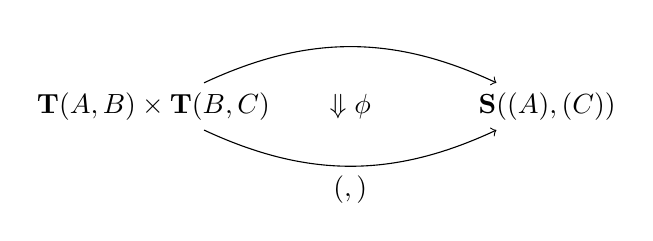
\begin{tikzpicture}
\node(1) at (0,0) {${\bf T}(A,B) \times {\bf T}(B,C)$};
\node(2) at (5,0) {${\bf S}(\cT(A),\cT(C))$};
\draw[->] (1) to[in=155, out=25] node[above]{$\cT \comp $} (2); 
\draw[->] (1) to[in=-155, out=-25] node[below]{$ \comp (\cT,\cT)$} (2); 
\node at (2.5,0) {$\Downarrow \phi \iso$};
\end{tikzpicture}
\end{align}
\item For every object $A$ of {\bf T} a tight transformation
\begin{align}
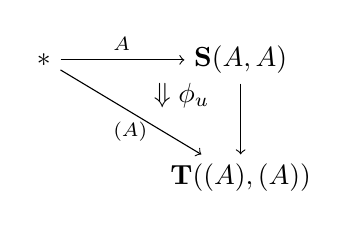
\begin{tikzpicture}[xscale=.5, yscale=.3]
\node(1) at (0,0) {$*$};
\node(2) at (5,0) {${\bf S}(A,A)$};
\node(3) at (5,-5) {${\bf T}(\cT(A),\cT(A))$};
\draw[->] (1) to node[above]{$\looseid_{A}$} (2); 
\draw[->] (1) to node[below]{$\looseid_{\cT(A)}$} (3);
\draw[->] (2) to node[right]{$\cT$} (3); 
\node at (3.5,-1.5) {$\Downarrow \phi_u \iso$};
\end{tikzpicture}
\end{align}
\item The usual coherence diagrams, Definition 10 of~\cite{nick:tricatsbook} commute.
\end{enumerate}
\end{defn}

%As any bicategory can be regarded as a double category with only identity tight 1-morphisms, any iconic tricategory can be regarded as a locally cubical bicategory and any iconic trifunctor can be regarded as a functor of locally cubical bicategories.

Let $\cDbl_f$ denote the sub-2-category of $\cDbl$ containing the double categories, all functors between them, and only transformations with loosely strong companions; we regard this as a locally cubical bicategory with only identity loose 2-morphisms and identity 3-cells.  The functor $\comp$ is defined on tight transformations as the Godement product. The pseudo double functor $\transid_A: * \rightarrow \cD bl(A,A)$ maps the cells in the trivial double category $*$ to the identity cells and morphisms in $\cD bl(A,A)$. 

As described in~\cite{gg:ldstr-tricat}, bicategories, pseudo functors, pseudo transformations, icons and cubical modifications also form a locally cubical bicategory. We will recall the definition of a cubical modification.

\begin{defn}
Let $F,G,H,K: \cD \rightarrow \cE$ be pseudo functors; let $\alpha: F \Rightarrow G$, $\beta: H \Rightarrow K$ be pseudo transformations; let $\gamma: F \Rightarrow H$, $\delta: G \Rightarrow K$ be icons. A cubical modification
\[
\begin{tikzpicture}
\node (tl) at (0,1) {$F$};
\node (tr) at (1,1) {$G$};
\node (bl) at (0,0) {$H$};
\node (br) at (1,0) {$K$};
\draw[doubletight] (tl) to node[above]{$\alpha$} (tr);
\draw[doubletight] (bl) to node[below]{$\beta$} (br);
\draw[doubletight] (tl) to node[left]{$\gamma$} (bl);
\draw[doubletight] (tr) to node[right]{$\delta$} (br);
\node at (.5,.5) {$\DDownarrow \Gamma$};
\end{tikzpicture}
\]
is given by a family of 2-cells $\Gamma_A: \alpha_A \RRightarrow \beta_A$ such that for every 1-cell $f:A \rightarrow B$ of $\cD$, the following equality holds.

 \begin{equation}
 \begin{aligned}
 \begin{tikzpicture}[scale=1.5]
 \node (tl) at (-1,1) {$FA$};
 \node (tm) at (0,1) {$FB$};
 \node (tr) at (1,1) {$GB$};
 \node (bl) at (-1,0) {$FA$};
 \node (bm) at (0,0) {$GA$};
 \node (br) at (01,0) {$GB$};
 \node (bl1) at (-1,-.7){$HA$};  
 \node (bm1) at (0,-.7) {$KA$};
 \node (br1) at (1,-.7) {$KB$}; 
 \draw[doubletight] (tm)  to node[above]{$\alpha_B$} (tr);
 \draw[doubleeq] (bm) to (bm1);
 \draw[doubletight] (bm) to node[above] {$Gf$}(br);
 \draw[doubleeq] (tr) to (br);
 \draw[doubleeq] (tl)  to  (tm);
 \draw[doubleeq] (tl) to (bl);
 \draw[doubletight] (tl) to node[above]{$Ff$}(tm);
 \draw[doubletight] (bl) to node[above]{$\alpha_A$}(bm);
 \node at (0,.5) {\footnotesize $\Downarrow \alpha_f$}; 
 \node at (0.5,-.3) {\footnotesize $\Downarrow \delta_f$}; 
  \node at (-0.5,-.3) {\footnotesize $\Downarrow \Gamma_A$};
 \draw[doubletight] (bl1)  to node[above]{$\beta_A$} (bm1);
 \draw[doubletight] (bm1) to  node[above]{$Kf$}(br1);
 \draw[doubleeq] (bl)  to (bl1);
 \draw[doubleeq] (br)  to (br1);
 \end{tikzpicture}
 \end{aligned}
 =
\begin{aligned}
 \begin{tikzpicture}[scale=1.5]
 \node (tl) at (-1,1) {$FA$};
 \node (tm) at (0,1) {$FB$};
 \node (tr) at (1,1) {$GB$};
 \node (bl) at (-1,0) {$HA$};
 \node (bm) at (0,0) {$HB$};
 \node (br) at (01,0) {$KB$};
 \node (bl1) at (-1,-.7){$HA$};  
 \node (bm1) at (0,-.7) {$KA$};
 \node (br1) at (1,-.7) {$KB$}; 
 \draw[doubletight] (tm)  to node[above]{$\alpha_B$} (tr);
 \draw[doubleeq] (tm) to (bm);
 \draw[doubletight] (bm) to node[above] {$\beta_B$}(br);
 \draw[doubleeq] (tr) to (br);
 \draw[doubleeq] (tl)  to  (tm);
 \draw[doubleeq] (tl) to (bl);
 \draw[doubletight] (tl) to node[above]{$Ff$}(tm);
 \draw[doubletight] (bl) to node[above]{$Hf$}(bm);
 \node at (-0.5,.5) {\footnotesize $\Downarrow \gamma_f$}; 
 \node at (0.5,.5) {\footnotesize $\Downarrow \Gamma_B$}; 
 \draw[doubletight] (bl1)  to node[above]{$\beta_A$} (bm1);
 \draw[doubletight] (bm1) to  node[above]{$Kf$}(br1);
 \draw[doubleeq] (bl)  to (bl1);
 \draw[doubleeq] (br)  to (br1);
 \node at (0,-0.3) {\footnotesize $\DDownarrow \beta_f$}; 
 \end{tikzpicture}
 \end{aligned}
\end{equation}

\end{defn}

The pseudo functor $\transid_A: * \rightarrow \cB icat(A,A)$ maps the cells in the trivial bicategory $*$ to the identity cells and morphisms of $\cB icat(A,A)$. 
The pseudofunctor $\comp$ is defined on functors as composition in the iconic tricategory $\cB icat$. On pseudo transformations and icons it is given by the Godement product. On cubical modifications it is defined below:

\begin{equation*}
\begin{aligned}
 \begin{tikzpicture}[scale=2]
 \node (tl) at (-1,1) {$FF'A$};
 \node (tm) at (0,1) {$GF'A$};
 \node (tr) at (1,1) {$GG'A$};
 \node (bl) at (-1,0) {$HF'A$};
 \node (bm) at (0,0) {$KF'A$};
 \node (br) at (01,0) {$KG'A$};
 \node (bl1) at (-1,-1){$HH'A$};  
 \node (bm1) at (0,-1) {$KH'A$};
 \node (br1) at (1,-1) {$KK'A$}; 
 \draw[doubletight] (tm)  to node[above]{$G(\alpha'_A)$} (tr);
 \draw[doubleeq] (tm) to (bm);
 \draw[doubletight] (bm) to node[above] {$K(\alpha'_A)$}(br);
 \draw[doubleeq] (tr) to (br);
 \draw[doubleeq] (tl)  to  (tm);
 \draw[doubleeq] (tl) to (bl);
  \draw[doubleeq] (bm) to (bm1);
 \draw[doubletight] (tl) to node[above]{$\alpha_{F'A}$}(tm);
 \draw[doubletight] (bl) to node[above]{$\beta_{F'A}$}(bm);
 \node at (-0.5,.5) {\footnotesize $\Downarrow \Gamma_{F'A}$}; 
 \node at (0.5,.5) {\footnotesize $\Downarrow \delta_{\alpha'_A}$}; 
 \draw[doubletight] (bl1)  to node[above]{$\beta_{H'A}$} (bm1);
 \draw[doubletight] (bm1) to  node[above]{$K(\beta'A)$}(br1);
 \draw[doubleeq] (bl)  to (bl1);
 \draw[doubleeq] (br)  to (br1);
 \node at (-.5,-0.5) {\footnotesize $=$}; 
\node at (.5,-0.5) {\footnotesize $\DDownarrow K\Gamma'_A$}; 
\end{tikzpicture}
\end{aligned}
\end{equation*}
%%%%%%%%%

Functoriality follows from naturality of the icons. Note that there are several canonical ways to define this composition on cubical modifications, by choosing different versions of the Godement product.  


%An icon is, morally speaking, an oplax transformation whose 1-cell components are all identities; but as noted by~\cite{lack:icons} this can be reexpressed without referring to these identity morphisms at all, yielding a definition that is easier to work with (because identity 1-cells in a bicategory are not strict).

%\begin{defn}
%Let $\cD, \cE$ be bicategories, and let $F,G: \cD \rightarrow \cE$ be pseudo functors. An {\bf icon} $\alpha: F \Rightarrow G$ is given by a family of 2-cells $\alpha_f : Ff \Rightarrow Gf$ indexed by the 1-cells of $\cD$, which are natural in $f$ and such that for all objects $A, B, C$ and 1-cells $A \xrightarrow{f} B \xrightarrow{g} C$ the following diagrams commute:
%\[
%\begin{tikzpicture}[xscale=1.5]
%\node (tl) at (0,1) {$\id_{FA}$};
%\node (tr) at (1,1) {$F \id_A$};
%\node (bl) at (0,0) {$\id_{GA}$};
%\node (br) at (1,0) {$G\id_A$};
%\draw[doubletight] (tl) to node[above]{$\iso$} (tr);
%\draw[doubletight] (bl) to node[below]{$\iso$} (br);
%\draw[doubleeq] (tl) to (bl);
%\draw[doubletight] (tr) to node[right]{$\alpha_{\id_A}$} (br);
%\end{tikzpicture}\qquad
%\begin{tikzpicture}[xscale=2]
%\node (tl) at (0,1) {$Fg  Ff$};
%\node (tr) at (1,1) {$F(gf)$};
%\node (bl) at (0,0) {$Gg Gf$};
%\node (br) at (1,0) {$G(gf)$};
%\draw[doubletight] (tl) to node[above]{$\iso$} (tr);
%\draw[doubletight] (bl) to node[below]{$\iso$} (br);
%\draw[doubletight] (tl) to node[left]{$\alpha_g \alpha_f$}(bl);
%\draw[doubletight] (tr) to node[right]{$\alpha_{gf}$} (br);
%\end{tikzpicture}
%\]
%\end{defn}



%That is, it is a structure \bS\ with objects, hom-bicategories $\bS(A,B)$, composition functors $\bS(B,C)\times \bS(A,B)$, identities $1_A \in \bS(A,A)$, and associativity and unitality \emph{icons} that satisfy the usual pentagon and triangle identities.
%(There is no room for any higher coherence, since the data of an icon consists of 2-cells only.)
%In particular, composition of 1-cells (objects of $\bS(A,B)$) is strictly associative, though the associativity for horizonatl composition of 2-cells is mediated by an icon.

%Similarly, we have the notion of \textbf{iconic functor}, namely an \Icon-enriched functor of bicategories.
%We can write this explicitly as follows.


\begin{thm}\label{thm:h-functor}
  There is a functor of locally cubical bicategories $\cH\maps \cDblf\to \cBicat$.
\end{thm}
\begin{proof}
Since any pseudo functor can be seen as a double functor between double categories with only identity tight 1-morphisms, each pseudo functor $\cH: \cDbl(\D,\E) \rightarrow \cBicat(\cH\D, \cH \E)$ corresponds to a pseudo double functor $\fH: \fDblf(\D,\E) \rightarrow \fBicat(\fH\D, \fH \E)$. Consequently, the first two requirements in \autoref{def:Iconfunc} are satisfied by Theorems \ref{thm:1-func} and \ref{thm:h-locfr}.
The third requirement amounts to the existence of a tight transformation $\phi\maps \behat * \alhat \iso \widehat{\be*\al}$ for every pair of transformations with loosely strong companions 

  \[\vcenter{\xymatrix{\lC \rtwocell^F_G{\al} & \lD \rtwocell^H_K{\be}
      & \lE}}\]
      
      such that 
%
 \begin{equation}
        \vcenter{\xymatrix@-.5pc{
        1_{{\cH}H \odot {\cH}F} \ar[r]\ar[d]_{=} &
        \hat{1}_{H}* \hat{1}_{F}\ar[d]^{\phi}\\
        1_{{\cH}(H \odot F)}\ar[r] &
        \widehat{1_{H} * 1_{F}}}} \quad\text{and}\quad       
    \vcenter{\xymatrix@-.5pc{
        \widehat{\gm\al}* \widehat{\de\be} \ar[r]\ar[d]_\phi &
        (\gmhat* \dehat)\circ(\alhat* \behat)\ar[d]^{\phi * \phi}\\
        \widehat{\gm\al* \de\be}\ar[r] &
        (\widehat{\gm* \de})\circ(\widehat{\al* \be})}}
  \end{equation}
commute. 
Here, we use the 'Godement product' $*$ of 2-cells in $\cDbl$.  

  Now by Lemmas \ref{thm:comp-compose} and
  \ref{thm:comp-func}, $(\behat *\alhat)_A = \behat_{GA} \circ
  H(\alhat_A)$ is a companion of $(\be*\al)_A = \be_{GA} \circ
  H(\al_A)$.  Therefore, we take the component $(\phi_{\alpha,\beta})_A$ to be
  \[\theta_{\behat_{GA} \circ H(\alhat_A),\, \widehat{\be*\al}_A}.\]
 As the other morphisms in the diagrams above are also $\theta$-isomorphisms, the equations hold by uniqueness of $\theta$-isomorphisms.
For the tight transformation  $\phi_u$ we can simply take the identity, since $\cH$ is strictly unital.
The coherence equations hold by uniqueness of $\theta$-isomorphisms.
\end{proof}

Our goal is to enhance this functor to act on ``monoidal objects''.
It is well-known that ``monoidal functors preserve monoid objects'', so our approach will be to categorify this: we will show that $\cH$ is monoidal, in an appropriate sense, and that monoidal functors of this sort preserve monoidal objects of the appropriate sort.

In fact, the monoidality of $\cH$ is easy to describe, because the monoidal structures of $\cDblf$ and $\cBicat$ are cartesian and very strict.

In general, if $\mathcal{V}$ is a monoidal 2-category with strict 2-categorical finite products (such as \cDbl), we say that a $\mathcal{V}$-enriched bicategory ${\bf B}$ has \textbf{finite products} when for each two objects $C,D \in {\bf B}$ there is an object $C\times D$ with projections $C\times D\to C$ and $C\times D\to D$ (i.e.\ morphisms $I\to \mathbf{B}(C\times D,C)$ and $I\to \mathbf{B}(C\times D,D)$ in \cV) inducing an \emph{isomorphism} in $\mathcal{V}$ (not merely an equivalence):
%
\begin{align}
{\bf B}(A, C \times D) \xrightarrow{\cong} {\bf B}(A,C) \times {\bf B}(A,D)
\end{align}
and similarly there is a strict terminal object $\ast$ such that $\bB(A,\ast)$ is strictly terminal in \cV\ for all $A$.
This holds for \cBicat\ and \cDblf, because cartesian products of bicategories and double categories are simply componentwise, and all the morphisms in \cBicat\ and \cDblf\ (no matter how weak) are defined in terms of data in their targets.

Similarly, we say that a functor $F$ of \cV-enriched bicategories \textbf{preserves products} if it takes the terminal object to a terminal object and pairs of product projections $A \leftarrow A\times B \to B$ to pairs of product projections (in the above strict sense).

\begin{thm}
The functor of locally cubical bicategories $\cH: \cDblf \rightarrow \cBicat$ preserves products.
\end{thm}
\begin{proof}
Since $\cH$ merely forgets a part of the double categories and double functors, we have simple equalities
$\cH(\mathbb{D} \times \mathbb{E}) = \cH(\mathbb{D}) \times \cH(\mathbb{E})$, and the product projections are likewise preserved.
The case of the terminal object is likewise easy.
\end{proof}

